\documentclass[.../bericht]{subfilies}

\begin{document}

\chapter{Physical background}


  \section{Forces on the particles}
  \label{sec:forces}

    There are several forces affecting particles suspended in a solution. Most relevant for this experiment are the gravitational, the electrostatic double layer, the Van der Waals and the light force (the latter when using the optical tweezers).
    \medskip

    \textbf{Gravitational force:}\\
    The particles interact with the gravitational field of the earth. If their density is higher than the density of the solution that they are suspended in, the particles sink. In front of a wall, where the individual particle is affected by a repulsive force, a potential well forms.  The gravitational potential $V_\mathrm{G}$ can be described as
    \begin{align}
    V_\mathrm{G}=\frac{4\pi R^3}{3}g(\rho_\mathrm{p}-\rho_\mathrm{m})z=F_\mathrm{G}z,
    \end{align}
    with the density of the particle $\rho_\mathrm{p}$ and of the medium $\rho_\mathrm{m}$, the earth acceleration $g$, the particles radius $R$ and the distance from the wall $z$.
    \medskip

    \textbf{Eletrostatic double layer force:}\\
    The eletrostatic double layer force accounts for the repulsion between particles with the same charge and attraction between those particles of opposite charge. In this experiment, it describes the interaction between particles and the wall. If the particles are suspended in an electrolyte solution, as is the case here, the Poisson equation describes the relation between the electrostatic potential $\Phi (\vec{r})$ and the elementary charge $e$, $\vec{r}$ being the distance between the two interacting particles. The equation is given by
    \begin{align*}
    \Delta \Phi (\vec{r})=-\frac{e^2}{\epsilon k_\mathrm{B} T}(\underbrace{\rho_+(\vec{r})+\rho_-(\vec{r})}_{\rho(\vec{r})},
    \end{align*}
    where $\rho_+(\vec{r})$ ist the cation and $\rho_-(\vec{r})$ the anion concentration, $\epsilon$ the permittivity, $k_\mathrm{B}$ the Boltzmann constant and $T$ the temperature.

    If the two concentrations are symmetrical, as is the case for monovalent electrolytes like KBr, the Poisson-Boltzmann equation takes the form
    \begin{align*}
    \Delta \Phi= \frac{\beta e^2}{\epsilon}2\rho_+ \cdot\sinh\Phi= \underbrace{\frac{e^2}{\epsilon k_\mathrm{B} T}\sum_i \rho_i q_i^2}_{=\kappa^2} \cdot \sinh\Phi
    \end{align*}
    using the inverse Debye length $\kappa$, with $q_i$ as the ion charge and $r\in G$, $G$ being the area which is neither particle nor surface. Introducing the surface charge density of the particles particles $\sigma_\mathrm{p}$ and of the wall $\sigma_\mathrm{w}$ and $z$ as the distance between particle surface and wall yields
    \begin{align*}
    \beta V_{dl}(z)=\frac{64\pi \epsilon a}{\beta e^2} \gamma_p \gamma_w e^{-\kappa(z)}, \\
    \gamma_\mathrm{w/p}=\tanh \left[ \frac{1}{2}\sinh^{-1}  \left( \frac{\beta e \sigma_\mathrm{w/p}}{2\epsilon \kappa } \right) \right],
    \end{align*}
    with $\beta=1/k_\mathrm{B} T$ as known from thermodynamics.
    \medskip

    \textbf{Van der Waals force:}\\
    In comparison to the previously described electrostatic force, the Van der Waals force is much weaker. Moreover, it occurs mostly as an attractive force in nature. Microscopically, it is derived from the interactions between the fluctuating dipolmoments of the particles. Integration of the particle-particle and the particle-wall Van der Waals force over the sphere wall symmetry of this experiment provides
    \begin{align}
    \beta V_{disp}(z)=\frac{A(z)}{6k_B T}\left(\frac{2R}{z}\frac{z+R}{z+2R}-\ln\frac{z+2R}{z}\right),
    \end{align}
    with the distance between particle surface and wall $z$, $R$ the particle radius and $A(z)$ the Hamaker constant.
    \medskip

    \textbf{Light force with optical tweezers:}\\
    Counteracting some of the previously mentioned forces, optical tweezers can be used to hold particles in place by utilizing the light force. The light force accounts for the impulses of the icident photons being transferred to the particle when absorbing or reflecting the photons.

    To keep it simple, a one dimensional system is regarded. The graviational force acting in negative $x$-direction $\vec{F}_\mathrm{G}^x$ can be counteracted by light force in positive $x$-direction $\vec{F}_\mathrm{L}^x$ to keep a particle floating at $x=x_0=const.$ yielding
    \begin{equation*}
    \vec{F}_\mathrm{G}^x=-\vec{F}_\mathrm{L}^x.
    \end{equation*}
    But optical tweezers can also hold dielectric particles in place against forces perpendicular to the light beam. To this end, a slightly focalised laser beam is utilized which holds the particle in the focus point as illustrated in \ref{fig:tweezer}.

    \begin{figure}[tb]
    \centering
    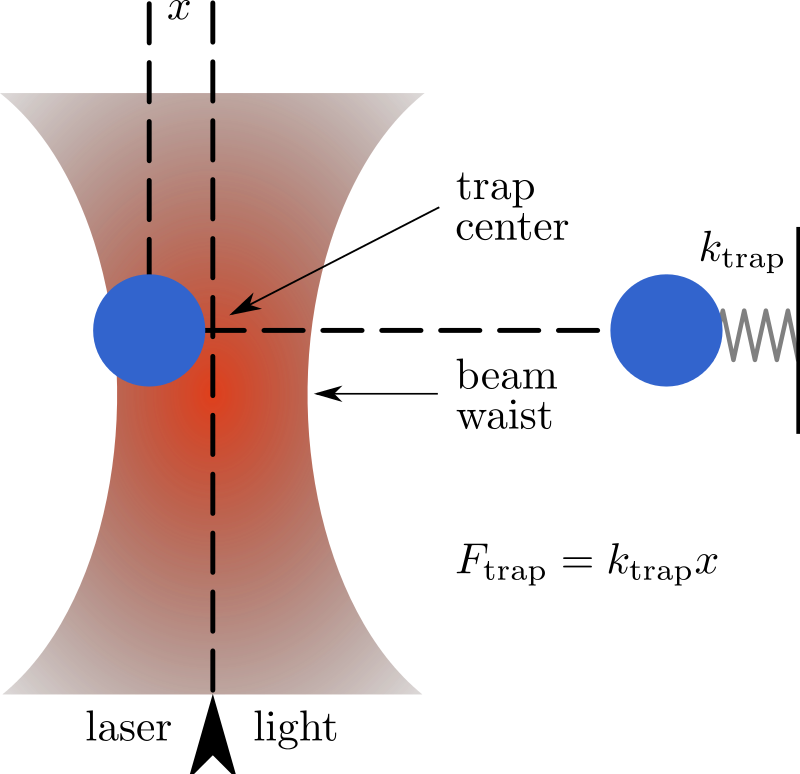
\includegraphics[width=0.5\textwidth]{figures/opticaltweezer}
    \caption{Particle trapped by an optical tweezer. The dielectric particle gravitates towards the beam center slightly above the beam waist. \cite{wiki:optical-tweezers}}
     \label{fig:tweezer}
    \end{figure}

    The force which moves the particle towards the beam's center is called the gradient force. It only moves the particle towards the center, if the refractive index of the particle is larger then the one of the solution in which the particle is suspended, though. If this is the case and there is an intensity gradient, the gradient force moves the particle towards the point of the highest intensity. The procces is similar to a dielectric being sucked into a capacitor. With a strong focus point it is also possible for the gradient force to override the light force if they have opposite directions. For optical tweezers in $x$- and $y$-direction the potentials are
    \begin{align}
    V_{\nabla,x}(x)=C_xPx^2\\
    V_{\nabla,y}(y)=C_yPy^2
    \end{align}
    with the laser power $P$ and the parameter $C$ depending on particle size, focus radius, refractive indices and more. \\
    Finally, for the $z$ direction the light force and the gravitational force add up to
    \begin{align}
    F_\mathrm{G,eff}^z=F_\mathrm{L}^z+F_\mathrm{G}^z.
    \end{align}
    \cite{helden}

    \section{Brownian motion}
    \label{sec:brownian-motion}

      The motion of particles suspended in a fluid resulting from their collision with fast moving molecules (or atoms) of the fluid is called the \textit{Brownian motion}.

      Within a fluid in thermal equilibrium at a given temperature, no preferential direction of flow exists. Therefore, the movement of the fluid's molecules is random yielding no linear or angular momenta over time. Sufficiently small particles suspended in this fluid move in random patterns, too, changing their velocities $\vec{v}$ upon colliding with one of the fluid's molecules. As a matter of fact, the observation has been deemed evidence for the existence of individual water (fluid) molecules.

      Because of the sheer number of involved fluid molecules, the many-body interactions resulting in the \textit{Brownian motion} cannot be solved relying only on classical mechanics. To put a number to it, the number of collisions of a single particle suspended in the fluid (a so called \textit{Brownian particles}) with the fluid molecules is roughly of the order $10^{14}$. Therefore, among others, Albert Einstein produced a probabilistic model using statistical mechanics. Einstein started by formulating a diffusion equation for the \textit{Brownian particle}. To this end, he regarded a one dimensional $x$-space with the origin at the initial position of the modelled \textit{Brownian particles}. Assuming the conservation of the number of fluid molecules and introducing the density function $\varphi(\Delta)$, with the random variable $\Delta$, he expanded the \textit{Brownian particle} density $\rho$ at a time $t + \tau$ in a Taylor series
      \begin{align*}
        \rho (x,t) + \tau \pdv{\rho (x)}{t}+\cdots=\rho (x,t+\tau )&= \rho (x,t)\cdot \int_{-\infty}^{\infty} \varphi (\Delta )\mathrm{d}\Delta \\
        &=\rho(x,t)\cdot\int_{-\infty}^{\infty} \varphi (\Delta ) \mathrm{d}\Delta  -\pdv{\rho}{ x}\cdot \int_{-\infty}^\infty \Delta \varphi (\Delta )\mathrm{d} \Delta \\
        &\quad + \pdv[2]{\rho}{x}\cdot \int_{-\infty}^{\infty} \frac{\Delta^2}{2} \varphi (\Delta ) \mathrm{d} \Delta + \cdots \\
        &=\rho(x,t)\cdot 1 +0+\pdv[2]{\rho}{x}\cdot \int_{-\infty}^{\infty} \frac{\Delta^2}{2}\varphi(\Delta ) \mathrm{d}\Delta +\cdots.
      \end{align*}
      While the integral in the second line equals one by definition of the probability, terms with even partials vanish due to symmetry of the 1D space. The above equation is leads to
      \begin{align}
        \pdv{\rho}{t}&\approx\pdv[2]{\rho}{x}\cdot \int_{-\infty}^{\infty} \frac{\Delta^2}{2\tau} \varphi ( \Delta) \mathrm{d}\Delta \nonumber  \\
        &=D\cdot \pdv[2]{\rho}{x}  \label{eq:diffusion-equation}
      \end{align}
      if only terms of $\Delta$ with orders smaller than 2 are regarded and using the \textit{mass diffusivity} or \textit{diffusion coefficient}
      \begin{equation}
        D=\int_{-\infty}^{\infty} \frac{\Delta^2}{2\tau} \varphi ( \Delta) \mathrm{d}\Delta.
        \label{eq:diffusion-coefficient}
      \end{equation}
      \cite{wiki:brownian-motion}


      \subsection{Brownian motion in proximity of the cavity walls}
      \label{subsec:brownian-wall}

        In \cref{sec:brownian-motion}, only the fluid's molecules surrounding the \textit{Brownian particles} have been taken into account for the diffusion equation \cref{eq:diffusion-equation}. When the fluid is confined in a cavity though, the cavity's walls affect the flow of the fluid. This statement can be proven by simply regarding a fluid molecule or \textit{Brownian particle} next the cavity wall. It's motion's component orthogonal to the wall is limited to one direction which is away from the wall. The interaction between the confining walls and the particles is called \textit{hydrodynamic interaction}.

        The mathematical description of this phenomenon makes use of distance $z$ dependent diffusion coefficients
        \begin{align}
          D_\parallel(z)&=D_0\left[ 1- \frac{9}{16} \left( \frac{a}{z+a}\right) + \frac{1}{8} \left( \frac{a}{z+a}\right)^3 - \frac{45}{256}\left( \frac{a}{z+a}\right)^4- \frac{1}{16}\left( \frac{a}{z+a}\right)^5+\cdots \right] \label{eq:D-parallel} \\
          D_\perp(z)&=D_0\left[ \frac{4}{3}\sinh (\alpha ) \sum_{n=0}^{\infty} \frac{n(n+1)}{(2n-1)(2n+3)}\left( \frac{2\sinh ((2n+1)\alpha )+(2n+1)\sinh (2\alpha )}{4\sinh^2 ((n+ \frac{1}{2})\alpha)-(2n+1)^2 \sinh^2 (\alpha )} - 1 \right) \right]^{-1} \nonumber \\
          &\approx D_0\cdot \frac{6 \left( \frac{z}{a}\right)^2 + 2 \frac{z}{a}}{6\left( \frac{z}{a}\right)^2 + 9 \frac{z}{a} + 2} \label{eq:D-perp}
        \end{align}
         for the motion orthogonal ($\perp$) and parallel ($\parallel$) to the walls, where $z$ is the distance between particle and wall and $\alpha=\arccos \left( \frac{z+a}{a} \right)$. For the approximation of \cref{eq:D-perp} please refer to \cite{beavan}. The diffusion coefficients are plotted in \cref{fig:D-wall}. As expected from the thought experiment this section has been introduced with, $D_\perp (z=0)=0$, whereas $D_\parallel (z=0)\ne 0$. \cite{helden}

         \begin{figure}
           \centering
           \tikzsetnextfilename{D_walls}
           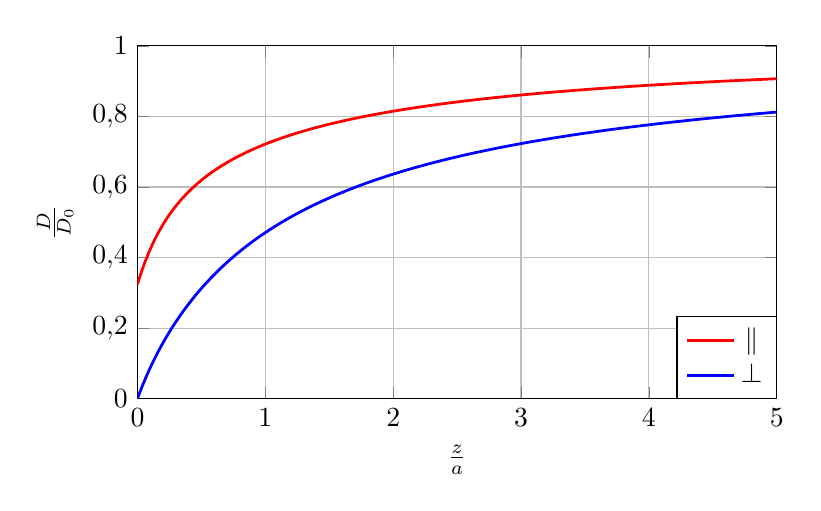
\begin{tikzpicture}
               \begin{axis}[
                 /tikz/line join=bevel,
                 width=0.8*\textwidth,
                 height=0.5*\textwidth,
                 grid,
                 legend style={at={(1,0)}, legend columns=1, anchor=south east},
                 every axis plot,
                 xmin = 0, xmax = 5,
                 ymin = 0, ymax = 1,
                 ylabel = {$\frac{D}{D_0}$},
                 xlabel = {$\frac{z}{a}$},
                 /pgf/number format/use comma,
                 /pgf/number format/1000 sep={},
                 ]
                 % Add plots
                 \addplot[domain=0.00001:5,samples=500, unbounded coords=discard, color=red, line width=1pt] {1-9/16*(x/(x^2+x))+1/8*(x/(x^2+x))^3-45/256*(x/(x^2+x))^4-1/16*(x/(x^2+x))^5};
                 \addlegendentry{$\parallel$}
                 \addplot[domain=0:5,samples=500, unbounded coords=discard, color=blue, line width=1pt] {(6*x^2+2*x)/(6*x^2+9*x+2)};
                 \addlegendentry{$\perp$}
               \end{axis}
           \end{tikzpicture}
           \caption{Distance dependent diffusion coefficients for a particle of diameter $a$ at a distance $z$ from the walls for parallel and perpendicular components of motion (compare \cref{subsec:brownian-wall}).}
           \label{fig:D-wall}
         \end{figure}


        \subsection{Langevin equation}

          A different approach to the \textit{Brownian motion} of colloidal particles respecting interactions with an interface makes use of the \textit{Langevin equation}. Herefore, the approach through  Langevin dynamics yields the equation
          \begin{equation*}
            \Delta \vec{r}=\frac{\vec{D}}{k_\mathrm{B}T}\cdot \vec{F}\Delta t+ \nabla \cdot \vec{D}\Delta t + \vec{X},
          \end{equation*}
          where $\vec{D}$ is the direction of motion dependent diffusion coefficient, $k_\mathrm{B}T$ the thermal energy, $\vec{F}$ the external force acting on the particle (comapre \cref{sec:forces}) and $\vec{X}$ is the Brownian contribution to $\Delta \vec{r}$. Moreover, $\vec{r}$ is the particles position and $\Delta t$ the time interval, which will be restricted later.

          The change of the particles position due to external forces $\vec{F}$ is the so called \textit{drift}, which makes the first term on the righthand side the \textit{drift-term}. As the diffusion coefficient depends on the particle's position in proximity of interfaces, the second term can be identified as the \textit{gradient term}. Finally, the third term describes the contribution of the \textit{Brownian motion}. As during the conducted experiment the measured particles will be trapped by optical tweezers, only the the component perpendicular to the surface of the cuvette needs to be regarded. Therefore, the above equation is written in scalar form
          \begin{equation}
            \Delta h = \frac{D}{k_\mathrm{B}T}F \Delta t + \frac{\mathrm{d}D}{\mathrm{d}h}\Delta t + \Delta h_\mathrm{Brownian},
            \label{eq:langevin-1d}
          \end{equation}
          $D$ and $F$ representing the normal components of the diffusion coefficient and the force vectors (regarding the surface of the cuvette), respectively, $\Delta h$ being the total change of distance between particle and the cuvette's wall during the time interval $\Delta t$.
          \begin{equation*}
            h_\mathrm{Brownian}=\chi \sqrt{2D\Delta t}
          \end{equation*}
           is therefore change of the distance between particle and interface due to the \textit{Brownian motion} during $\Delta t$, where $\chi$ is randomly chosen from a set of normally distributed numbers with a mean of zero and standard deviation of one. Using this identity, \cref{eq:langevin-1d} becomes
           \begin{equation*}
             \Delta h = \frac{D}{k_\mathrm{B}T}F\Delta t + \frac{\mathrm{d}D}{\mathrm{d}h}\Delta t + \chi \sqrt{2D\Delta t}.
           \end{equation*}
           For this equation to be physical, $\Delta t$ needs to be longer than the relaxation time of the \textit{Brownian fluctuations} and at the same time Sufficiently small as to be able to regard $D$ and $F$ as constant. Using $\Delta t \rightarrow 0 $ within these bounds, the \textit{Brownian term} is prominent as it only scales with $\sqrt{\Delta t}$, whereas the other two terms scale with $\Delta t$. This leads to $\Delta h$ being normally distributed with the variance
           \begin{equation}
             \sigma_{\Delta h}^2=2D\Delta t.
             \label{eq:variance-simple}
           \end{equation}
           Regarding the case where $t\rightarrow \infty$, the \textit{Brownian motion} as a fluctuation does not change the particles' positions effectively. The potential well trapping the particle $\phi (h)$ becomes prominent. Therefore, the time dependent variance is given by
           \begin{equation*}
             \sigma_{\Delta h}^2=\sigma_{\Delta h, \infty}^2 \left[ 1-\exp\left( - \frac{2D\Delta t}{\sigma_{\Delta h, \infty}}\right)\right],
           \end{equation*}
           $\sigma_{\Delta h,\infty}$ being the variance at large times. This is in accordance with \cref{eq:variance-simple} when Taylor expanding around $\Delta t = 0$. As the variance should reach zero for $\Delta t \rightarrow \infty$, the probability of a particle with initial position $h_0$ to being found at $h_0 +\Delta h$ is concluded to be
           \begin{equation*}
              p(h_0+ \Delta h)=A\exp\left( \frac{-\phi (h_0+\Delta h)}{k_\mathrm{B}T}\right).
           \end{equation*}
           Here, $A$ is a normalization constant and $\phi ( h_0 + \Delta h)$ the potential energy of the particle at position $h_0 + \Delta h$. For the form of the potential, the forces mentioned in \cref{sec:forces} must be respected. \cite{walz}



      \section{Evanescent field}
      \label{sec:evanenscent}

        To analyze the position fluctuations of the particles in the aqueous dispersion, an evanescent field is utilized. An evanescent field is a field of any kind, were there is no net energy flow in any given direction. In this experiment, this is achieved by total reflection. \\
        If  a lightbeam hits a transition between two media with the refraction indices $n_1$ for medium 1 and $n_2$ for medium 2 at the angle $\Theta_1$, part of it is refracted at the angle $\Theta_2$ and part of it is reflected at the angle $\Theta_1$. This relation is described by Snell's law
        \begin{equation*}
          n_1 \sin(\Theta_1)=n_2 \sin(\Theta_2).
        \end{equation*}
        If $n_1>n_2$, there is a critical angle $\Theta_c$ at which all the light is reflected and non of it transmits into medium 2 with
        \begin{align*}
          \Theta_c=\arcsin\left(\frac{n_2}{n_1}\right).
        \end{align*}
        Still, an exponentially decaying field component of the incident wave enters the second medium. As it decays exponentially, there is no energy flow and it is therefore an evanescent wave. The resulting field distribution in medium 2 is given by
        \begin{align*}
          E_r=E_0 \exp\left( -\frac{\beta}{2}z \right) \exp\left( i\frac{n_1}{n_2}\sin(\Theta_1)kx-i\omega t \right),
        \end{align*}
        $2/\beta$ being the characteristic decay length. This means that the wave decays with $\beta^{-1}$ in the medium and this decay is defined as
        \begin{align*}
          \beta^{-1}=\frac{\lambda_0}{4 \pi \sqrt{n_1^2 \sin^2\Theta_1-n_2^2}},
        \end{align*}
        which shows that the penetration depth diverges at the critical angle $(\Theta_1=\Theta_c)$ and the minimum penetration depth is
        \begin{equation*}
          \beta^{-1}=\frac{\lambda_0}{4 \pi \sqrt{n_1^2-n_2^2}}.
        \end{equation*}
        \cite{helden}


      \section{Determination of the potential form}
      \label{sec:determination}

        The following explanations are taken from \cite{anleitung}.

        The scattering intensity $I(z)$ depends, in the following manner, on the distance $z$ between the particle and the wall:
        \begin{align}
          \begin{split}
            I(z)=I_0\exp\left( -\beta z \right) \leftrightarrow z&=-\beta^{-1}\ln\left(\frac{I_z}{I_0}\right)\\
            &=-\beta^{-1}\ln I(z) + \underbrace{\beta^{-1}\ln I_0}_{=z_0}
          \end{split}
          \label{eq:I-von-z}
        \end{align}
        Where $\beta^{-1}$ is the penetration depth of the evanescent field and $I_0$ is the scatter intensity that results when particles and wall are in direct contact. Without knowing this constant, only relative distances can be determined, since $z_0$ can not be computed. The absolute distance is determined hydrodynamically in the second section of the evaluation; here $I_0 = 10$ is assumed arbitraily. The Boltzmann equation combines the distance-dependent probability distribution $p(z)$ with the interaction potential $V(z)$ between particle and wall:
        \begin{equation*}
          p(z)=p_0\exp\left( -\frac{V(z)}{k_\mathrm{B}T}\right) \leftrightarrow \frac{V(z)}{k_\mathrm{B}T}=-\ln\left(\frac{p(z)}{p_0}\right)
        \end{equation*}
        The distance-dependant probability distribution is calculated using \cref{eq:I-von-z}, and can then be converted into en intensity probability distribiution $N(I)$:
        \begin{equation*}
          p(z)=N(I)\frac{\mathrm{d}I}{\mathrm{d}z}=-\beta N(I)I(z),
        \end{equation*}
        where $N(I)$ is obtained directly from the measured data as a histogram. The resulting potential is then
        \begin{equation}
          \frac{V(z)}{k_\mathrm{B}T}=-\ln\left(\frac{-\beta N(I)I(z)}{p_0}\right)=-\ln\left[ N(I)I(z) \right]+\ln\left( -\frac{p_0}{\beta}\right).
          \label{eq:potential}
        \end{equation}
        Before creating the histogram, the background must first be subtracted from the measured data. This corresponds to the scatter signal in the absence of the particle. For this purpose, the particle can be pulled out of the field of view with the optical tweezers and the background at the measuring position can be determined directly (approximately $\SI{10}{\second}$ to $\SI{30}{\second}$ measurement averaged). The number of bins in the histogram determines the number of potential values that are calculated. The error on the calculated potential value decreases with increasing number of counts per bin. Approximately 100 bins represent a good compromise between a small error of the individual potential values on the one hand and good local resolution on the other. \Cref{eq:potential} potential already has the correct shape, but not yet the correct absolute distance from the surface.

      \section{Hydrodynamic evaluation}
      \label{sec:hydrodynamic}

        This section is taken from \cite{anleitung}, too.

        For the determination of the potential shape, only the probability distribution has so far been used. However, much more information is available in the measurement data. An analysis of the dynamics of the measured data provides information on the distance dependence of the diffusion coefficient and also allows the determination of the absolute distance. The 3D diffusion coefficient (far from the surface), $D_0$ is described by the Stokes-Einstein equation
        \begin{equation*}
          D_0=\frac{k_\mathrm{B}T}{6\pi\eta R},
        \end{equation*}
        where $\eta$ is the vescosity of the liquid and $R$ corresponds to the particule's radius. In the vincinity of a wall, where the liquid molecules can not move (stick boundary conditions), the diffusion coefficient becomes distance-dependent and anisotropic (compare \cref{subsec:brownian-wall}). The distance-dependent diffusion coefficient for diffusion perpendicular to the wall $D_\perp$ was calculated analytically by Brenner as an infinite series \cite{2}. This series can be approximated very well for small distances $z<R$ to
        \begin{equation}
          D_\perp = \frac{D_0}{\frac{R}{z}+0,2\ln\left(\frac{R}{z}\right) + 0,9712}.
          \label{eq:d-perp-sheet}
        \end{equation}
        Considering the solution of the Langevin equation for a spherical particle near a wall, the distance-dependent diffusion coefficient can also be determined from the measured trajectory of the particle \cite{4}. To do this, the following procedure is applied:
        \medskip

        \begin{enumerate}
          \item The measured intensity data are converted into distances, whereby an arbitrary value is initially assumed for the scatter intensity at the contact of particle and wall ($I_0$ in \cref{eq:I-von-z}). The maximum input voltage of the A/D card of $\SI{10}{\volt}$ is for example a realistic starting value for $I_0$.
          \item For the analysis of the dynamics, the measured trajectory is divided into about 20 intervals $a_j$ . For each $a_j$ , a histogram of the distance changes $\Delta z_i$ is generated within a certain time interval $\Delta t$. That under the condition that the $i$-th distance value $z_i$ measured in the trajectory is in the interval $a_j$, $z_i = z_{i+k} - z_i$ is calculated and entered into the histogram. The time interval $t = k \delta t_\mathrm{mess}$ is necessarily an integer multiple of the measurement interval $\delta t_\mathrm{mess}$ and $k = 1,2$, in order not to average over too long time intervals. Neglecting the effects of the interaction potential (curvature), a Gaussian distribution of $p$ the distance changes is to be expected, whose width is $\sigma_{z_i ,\Delta t} = \sqrt{2D_{z_i} \Delta t}$. In principle, $D_{(z_i)}$ can already be determined from the fit parameter $\sigma_{(z_i,t)}$ for a certain $\Delta t$. However, a smaller measurement error is obtained if $\sigma_{(z_i ,t)}$ against $\Delta t$, and  $D_{(z_i)}$ is determined from the slope \cite{4}.
          \item The unknown parameter $I_0$ is now adapted such that the distance-dependent diffusion coefficient $D_z$ coincide with the theoretical predictions from \cref{eq:d-perp-sheet} ($\eta$ and $a$ are known). From this follows the correct absolute particle wall distance for the potential.
        \end{enumerate}
        In the practice of the experiment, the described evaluation is implemented by a predetermined MatLab routine, in which only $I_0$ has to be adapted as a parameter.










\end{document}
